\documentclass[hidelinks,12pt]{article}
\usepackage[left=0.25cm,top=1cm,right=0.25cm,bottom=1cm]{geometry}
%\usepackage[landscape]{geometry}
\textwidth = 20cm
\hoffset = -1cm
\usepackage[utf8]{inputenc}
\usepackage[spanish,es-tabla, es-lcroman]{babel}
\usepackage[autostyle,spanish=mexican]{csquotes}
\usepackage[tbtags]{amsmath}
\usepackage{nccmath}
\usepackage{amsthm}
\usepackage{amssymb}
\usepackage{mathrsfs}
\usepackage{graphicx}
\usepackage{subfig}
\usepackage{caption}
%\usepackage{subcaption}
\usepackage{standalone}
\usepackage[outdir=./Imagenes/]{epstopdf}
\usepackage{siunitx}
\usepackage{physics}
\usepackage{color}
\usepackage{float}
\usepackage{hyperref}
\usepackage{multicol}
\usepackage{multirow}
%\usepackage{milista}
\usepackage{anyfontsize}
\usepackage{anysize}
%\usepackage{enumerate}
\usepackage[shortlabels]{enumitem}
\usepackage{capt-of}
\usepackage{bm}
\usepackage{mdframed}
\usepackage{relsize}
\usepackage{placeins}
\usepackage{empheq}
\usepackage{cancel}
\usepackage{pdfpages}
\usepackage{wrapfig}
\usepackage[flushleft]{threeparttable}
\usepackage{makecell}
\usepackage{fancyhdr}
\usepackage{tikz}
\usepackage{bigints}
\usepackage{menukeys}
\usepackage{tcolorbox}
\tcbuselibrary{breakable}
\usepackage{scalerel}
\usepackage{pgfplots}
\usepackage{pdflscape}
\pgfplotsset{compat=1.16}
\spanishdecimal{.}
\renewcommand{\baselinestretch}{1.5} 
\renewcommand\labelenumii{\theenumi.{\arabic{enumii}})}

\newcommand{\python}{\texttt{python}}
\newcommand{\textoazul}[1]{\textcolor{blue}{#1}}
\newcommand{\azulfuerte}[1]{\textcolor{blue}{\textbf{#1}}}
\newcommand{\funcionazul}[1]{\textcolor{blue}{\textbf{\texttt{#1}}}}

\newcommand{\pderivada}[1]{\ensuremath{{#1}^{\prime}}}
\newcommand{\sderivada}[1]{\ensuremath{{#1}^{\prime \prime}}}
\newcommand{\tderivada}[1]{\ensuremath{{#1}^{\prime \prime \prime}}}
\newcommand{\nderivada}[2]{\ensuremath{{#1}^{(#2)}}}


\newtheorem{defi}{{\it Definición}}[section]
\newtheorem{teo}{{\it Teorema}}[section]
\newtheorem{ejemplo}{{\it Ejemplo}}[section]
\newtheorem{propiedad}{{\it Propiedad}}[section]
\newtheorem{lema}{{\it Lema}}[section]
\newtheorem{cor}{Corolario}
\newtheorem{ejer}{Ejercicio}[section]

\newlist{milista}{enumerate}{2}
\setlist[milista,1]{label=\arabic*)}
\setlist[milista,2]{label=\arabic{milistai}.\arabic*)}
\newlength{\depthofsumsign}
\setlength{\depthofsumsign}{\depthof{$\sum$}}
\newcommand{\nsum}[1][1.4]{% only for \displaystyle
    \mathop{%
        \raisebox
            {-#1\depthofsumsign+1\depthofsumsign}
            {\scalebox
                {#1}
                {$\displaystyle\sum$}%
            }
    }
}
\def\scaleint#1{\vcenter{\hbox{\scaleto[3ex]{\displaystyle\int}{#1}}}}
\def\scaleoint#1{\vcenter{\hbox{\scaleto[3ex]{\displaystyle\oint}{#1}}}}
\def\scaleiiint#1{\vcenter{\hbox{\scaleto[3ex]{\displaystyle\iiint}{#1}}}}
\def\bs{\mkern-12mu}

\newcommand{\Cancel}[2][black]{{\color{#1}\cancel{\color{black}#2}}}


\usepackage{minted}

\author{M. en C. Gustavo Contreras Mayén. \texttt{curso.fisica.comp@gmail.com}\\
M. en C. Abraham Lima Buendía. \texttt{abraham3081@ciencias.unam.mx}}
\title{Ejercicios para el Tema 0 - Repaso de python \\ {\large Curso Física Computacional}}
\date{ }
\begin{document}

\maketitle
\fontsize{12}{12}\selectfont

Los siguientes ejercicios permitirán aplicar lo que se ha visto en esta primera semana del curso, son \emph{ejercicios opcionales}, no forman parte de la evaluación, si los resuelves y envías en Moodle, se te regresarán con comentarios y observaciones. Ocupa una notebook de Jupyter para resolver cada ejercicio, puedes identificarlos usando celdas Markdown.

\begin{enumerate}
\item Para darnos cuenta de lo asombroso que puede ser \python, teclea \break \hfill \texttt{import antigravity}. Para apreciar la magnitud del ejercicio, debes de tener habilitada una conexión a internet.
\item Calcula el área de un triángulo de base $10$ y altura $12$.
\item Repite el ejercicio anterior, permitiendo al usuario que ingrese el valor de la base y el valor de la altura.
\item Nuevamente repite el ejercicio anterior, ahora utilizando una función.
\item Escribe un código que calcule la distancia entre dos puntos $(x_{1}, y_{1})$ y $(x_{2}, y_{2})$, el programa deberá de ejecutarse hasta que el usuario teclee \textit{adios} al momento de ingresar el valor para $x_{1}$.
\item Aunque se considera que un año tiene $365$ días, una cifra más exacta es $365.24$ días. Como consecuencia, si mantuviéramos el año estándar de $365$ días, perderíamos gradualmente esa fracción del día con el tiempo, y las estaciones y otros eventos astronómicos no ocurrirían como se esperaba. Para mantener la escala de tiempo al día, un \textit{año bisiesto} es un año que incluye un día adicional, el $29$ de febrero, para mantener la escala de tiempo al día.
\par
Los años bisiestos ocurren en años que son exactamente divisibles por $4$, a menos que sea exactamente divisible por $100$, a menos que sea divisible por $400$. Por ejemplo, el año $2004$ es bisiesto, el año $1900$ no es bisiesto y el año $2000$ es un año bisiesto. Calcula el número de años bisiestos entre los años $1500$ y $2030$.
\item El brillante matemático Srinivasa Ramanujan desarrolló una podera aproximación al valor de $\pi$. La expresión es la siguiente:
\begin{align*}
\dfrac{1}{\pi} \approx \dfrac{2 \, \sqrt{2}}{9801} \, \nsum_{k=0}^{N} \dfrac{(4 \, k)! \, (1103 + 26390 \, k)}{(k \, !)^{4} \, (396)^{4 k}}
\end{align*}
Usa la fórmula de Ramanujan para $N = 0$ y $N = 1$ para aproximar a $\pi$. Compara la aproximación obtenida con el valor que devuelve \python{} para $\pi$. Ocupa la librería \texttt{math} para usar la función factorial y el valor de $\pi$.
\item Considera un triángulo con vértices $(0, 0)$, $(1, 0)$ y $(0, 1)$. Escribe una función con el nombre \texttt{punto\_triangulo(x, y)}, donde la salida será la cadena \enquote{por fuera} si el punto $(x, y)$ está fuera del triángulo, si el punto está exactamente en el borde del triángulo, la salida será \enquote{en el borde}, y la cadena \enquote{dentro}, si el punto está por dentro del triángulo.
\
\begin{minted}{python}
def punto_triangulo(x, y):
    # Escribe tu código aquí

    return posicion

# Salida "en el borde"
punto_triangulo(0.5, 0.5)

# Salida "dentro"
punto_triangulo(0.25, 0.25)

# Salida "por fuera"
punto_triangulo(5, 5)
\end{minted}
\item ¿Cuál será el valor de $y$ luego de que se ejecute el siguiente código? Primero intenta  resolverlo mentalmente, luego verifica tu resultado con el código.
\begin{minted}{python}
y = 0
for i in range(1000):
    for j in range(1000):
        if i == j:
            y += 1
\end{minted}
\item Sabemos del cálculo y la geometría que una \textit{cicloide} es la curva trazada por un punto situado en el borde de una rueda que se desliza sobre una superficie plana. Las coordenadas (x, y) de una cicloide generada a partir de una rueda con radio $r$, se pueden describir mediante las ecuaciones paramétricas:
\begin{align*}
x &= r (\varphi - \sin \varphi) \\[0.5em]
y &= r (1 - \cos \varphi)
\end{align*}
donde $\varphi$ es el número de radianes que ha recorrido la rueda.
\par
Genera una gráfica de la cicloide para $0 \leq \varphi \leq 2\pi$ usando incrementos de 1000 y con $r = 3$. Dale a tu gráfica un título y etiquetas, incluye la cuadrícula (grid) y modifica los límites de los ejes para que la trama sea ordenada y atractiva. La siguiente figura te puede orientar en el acabado de la gráfica.
\begin{figure}[H]
    \centering
    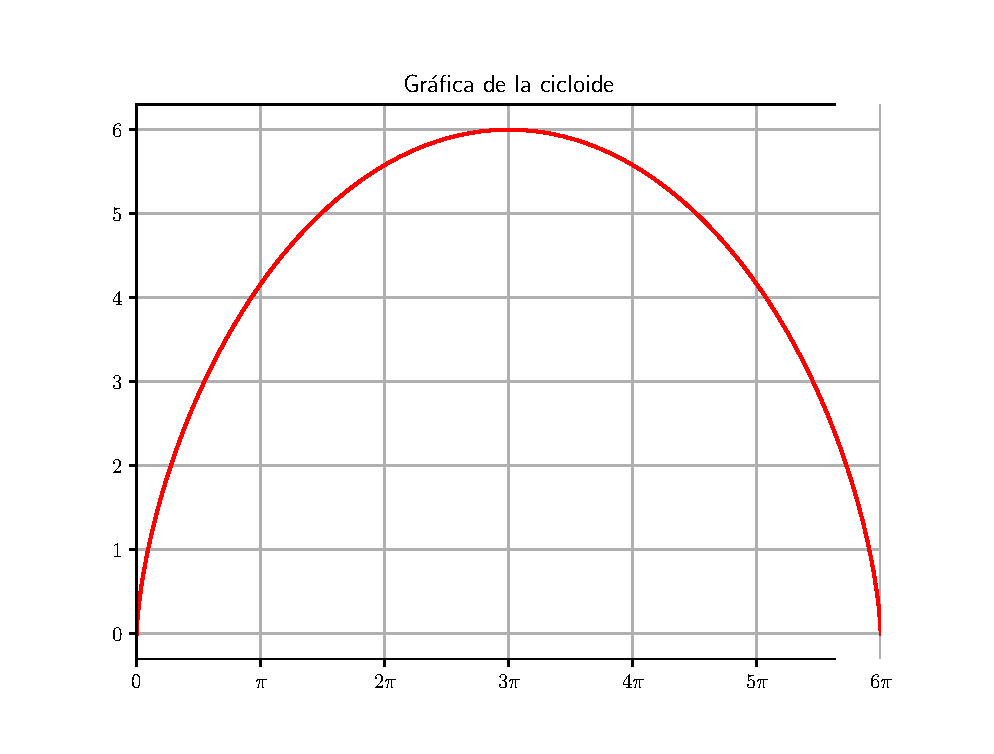
\includegraphics[scale=0.9]{Imagenes/Grafica_Cicloide.eps}
    \caption{Gráfica de la cicloide, la idea es que logres una imagen con la que se muestra.}
\end{figure}
\end{enumerate}
\end{document}